\documentclass[11pt]{article}
\usepackage{geometry}
\geometry{letterpaper, margin=1in}
\usepackage[utf8]{inputenc}
\usepackage{graphicx}
\usepackage{upgreek}
\usepackage{url}
\usepackage[T1]{fontenc}
\usepackage{amsmath}
\usepackage{minted}
\usepackage{scalerel}
\usepackage[colorinlistoftodos]{todonotes}
\usepackage[
backend=biber,
style=ieee,
sorting=none
]{biblatex}
 
\addbibresource{refs.bib}

\title{ECE532S Digital Systems Design \\ \vspace{0.4cm}
       \Large Tutorial 1 - Vivado Project Flow Basics \\ \vspace{0.4cm}
       \small Last Updated: Jan, 2020}
\author{ }
\date{ }


\begin{document}
\maketitle
\vspace{-1cm}

This tutorial guides you through the design flow of the Xilinx Vivado software to create a simple digital circuit using Verilog HDL. A typical design flow consists of creating model(s), creating user constraint file(s), creating a Vivado project, importing the created models, assigning created constraint file(s), optionally running behavioral simulation, synthesizing the design, implementing the design, generating the bitstream, and finally verifying the functionality in the hardware by downloading the generated bitstream file. You will go through the typical design flow targeting the Artix-100 based Nexys4 board. The typical design flow is shown in Figure~\ref{fig:design_flow}.

\begin{figure}[!h]
    \centering
    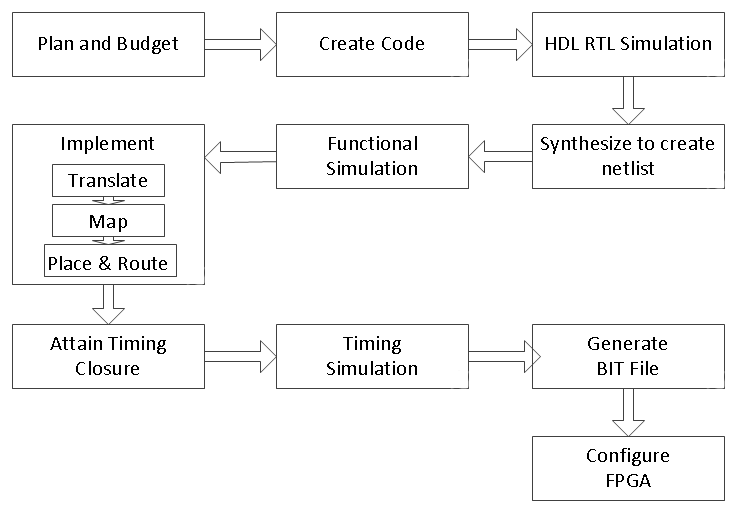
\includegraphics[width=0.9\textwidth]{images/design_flow.png}
    \caption{A typical Vivado design flow}
    \label{fig:design_flow}
\end{figure}




\section{Creating a Vivado Project}
\label{sec:create_proj}
Launch Vivado in order to create a new project. Note, if launching Vivado from a terminal, you may need to source a script located at:

\begin{verbatim}
    <Vivado Install Directory>/Xilinx/Vivado/<Vivado Version>/settings64.sh
\end{verbatim}

\noindent
For the UG machines for example, the script will be located in the following location:

\begin{verbatim}
    /cad1/Xilinx/Vivado/2018.1/settings.sh
\end{verbatim}

\noindent
To \textit{source} the script file, type the following command into the terminal and hit enter:

\begin{verbatim}
    source /cad1/Xilinx/Vivado/2018.1/settings.sh
\end{verbatim}

\noindent
After sourcing the script, launch Vivado by typing vivado into the terminal:

\begin{verbatim}
    vivado
\end{verbatim}

\noindent
If you're launching Vivado from a Windows machine, you should be able to find Vivado from the Start Menu and don't need to launch Vivado from the terminal. Note, if you do want to launch Vivado from the Command Shell on a Windows machine (perhaps to launch Vivado using a provided TCL script), follow the above steps but note that the extension for the script file will be \textit{.bat} rather than \textit{.sh}.

\begin{verbatim}
    <Vivado Install Directory>\Xilinx\Vivado\<Vivado Version>\settings64.bat
\end{verbatim}

\noindent
Once the Vivado GUI has opened, select \textbf{Create New Project} in order to start the project creation wizard. You will see a \textit{Create A New Vivado Project} dialog box; click \textbf{Next}. A zip file containing some necessary source files for this tutorial was distributed alongside this tutorial document, make sure the contents of that zip file are extracted to some directory in which you want to create your new project. In the \textit{project location} field of the current dialog, browse to the directory to which you extracted the project files. Enter \textbf{tutorial} in the \textit{project name} field and make sure that the \textit{Create project subdirectory} box is checked; click \textbf{Next}. See Figure~\ref{fig:new_proj_name} for an example.

\begin{figure}[!h]
    \centering
    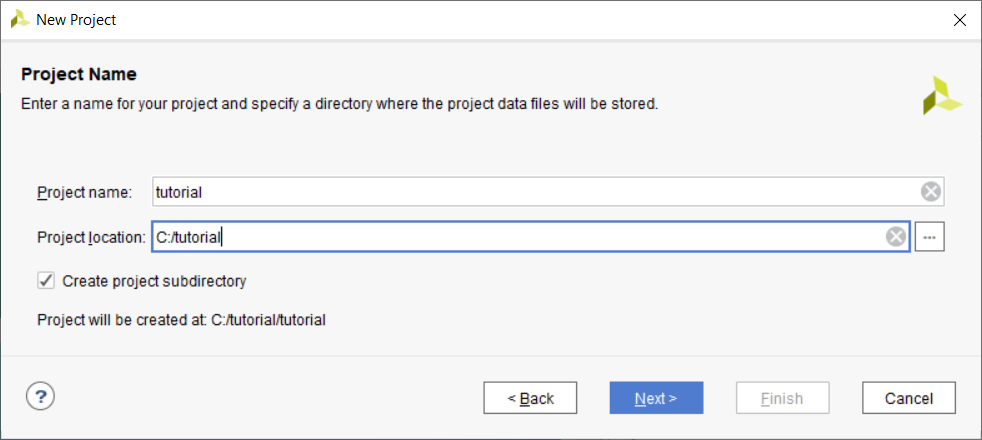
\includegraphics[width=0.9\textwidth]{images/new_proj_name.png}
    \caption{Project name and location entry}
    \label{fig:new_proj_name}
\end{figure}

In the next window of the project creation wizard, Select the \textbf{RTL Project} option in the \textit{Project Type} form, and click \textbf{Next}. Now we have the \textit{Add Sources} window. On this page, we add any source files that we have already created to the project. Select \textbf{Verilog} as the \textit{Target Language} and then click on the \textbf{Add Files…} button. From here you can browse to the location of any source you wish to add. For this tutorial, browse to the extracted files and select \textit{tutorial.v} and click \textbf{OK} to add that source to the project. Make sure to check the box labelled \textit{Copy sources into project} before proceeding to the next pane. This check box option copies any of the selected source files into the newly created project, which means changes to the source within the project will not effect the original file and, conversely, changes to the original file will not be seen by the project. In future projects, keep in mind whether or not this is the behaviour you'd like for your project and select the option accordingly. click \textbf{Next} to move to the next page. See Figure~\ref{fig:new_proj_src} for an example.

\begin{figure}[!h]
    \centering
    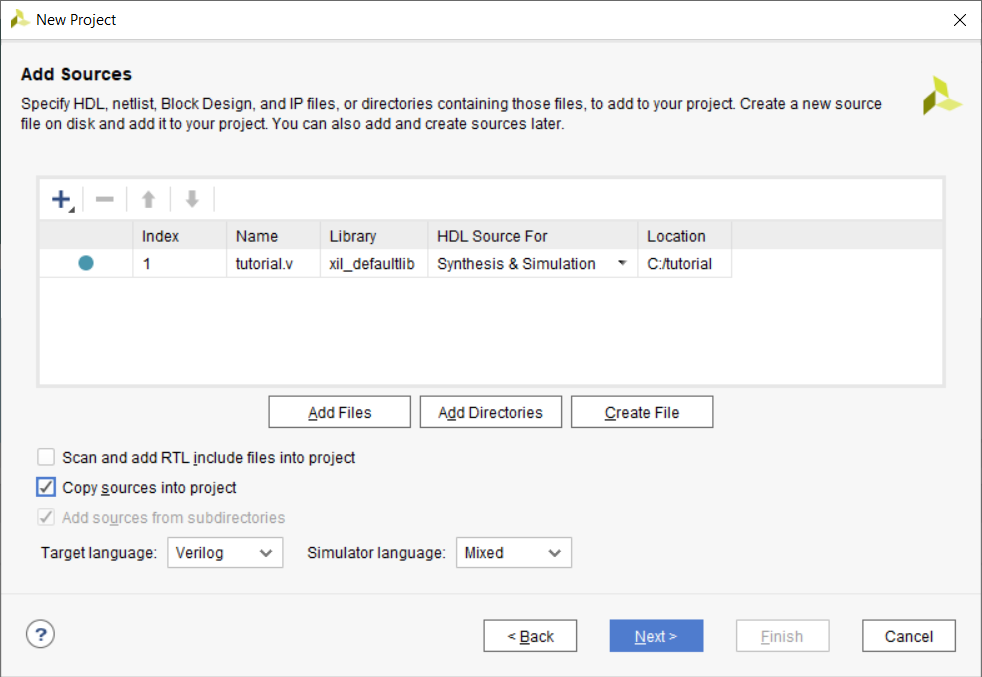
\includegraphics[width=0.9\textwidth]{images/new_proj_src.png}
    \caption{Project source selection window}
    \label{fig:new_proj_src}
\end{figure}

Now we have the \textit{Add Constraints} window. In FPGA projects, constraints are used to specify things like which signals ought to connect to specific pins on the FPGA, and the frequency of our external clock sources. For this tutorial, we've provided a constraints file (extension \textit{.xdc}).  Click on the \textbf{Add Files...} button and browse to the location of the extracted files. Select the \textit{tutorial.xdc} file and click \textbf{Open} (if necessary). Ensure that \textit{Copy constraints files into project} check box is selected (this option serves the same purpose as we discussed with the source files earlier). Click \textbf{Next} and proceed to \textit{Default Part} selection.

In the \textit{Default Part} form, using the \textbf{Parts} option and the various drop-down fields of the Filter section (or the search box), select the \textbf{XC7A100TCSG324-1} part. This corresponds to the FPGA part of the Nexsys DDR4 board (if you're using a Nexsys Video board, adjust this accordingly). See Figure~\ref{fig:new_proj_device} for an example. Note, while we used the \textit{Parts} option to select our part, a \textit{Boards} option is also available, which will select the appropriate part for the board you select in that list. The Nexsys boards aren't included in Xilinx's list of boards, though in later tutorials we'll go through how to add board files to the Vivado install such that Nexsys devices appear in the list. Note also that using the board option often allows us to avoid using a constraints file, since many of the constraints are defined in the board files themselves. For this tutorial, we'll stick to the \textit{Part} selection option. Click \textbf{Next} and then \textbf{Finish} in the last pane of the wizard to create the project.

\begin{figure}[!h]
    \centering
    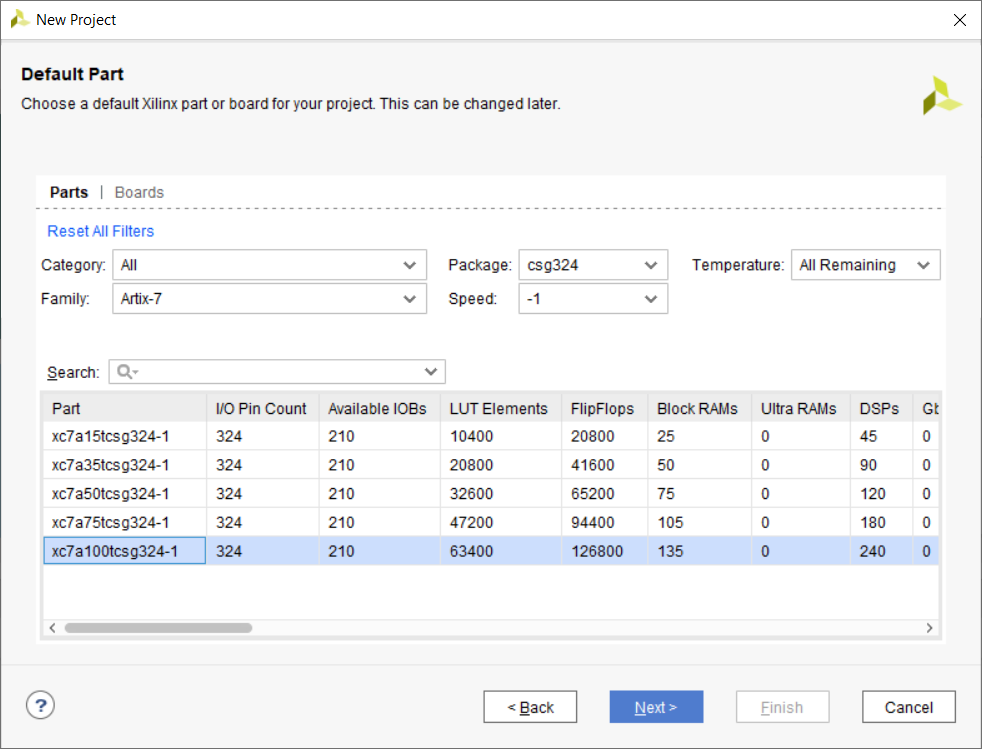
\includegraphics[width=0.9\textwidth]{images/new_proj_device.png}
    \caption{Default part selection window}
    \label{fig:new_proj_device}
\end{figure}




\section{Navigating the Vivado Project View}
\label{sec:navigating_vivado}
Once you have finished the project creation wizard, the Vivado \textit{Project Manager} view should be open for your newly created project. There are a number of different panes within this view that expose different features of Vivado or different aspects of the project on which you are working. Figure~\ref{fig:vivado_layout} shows the Vivado \textit{Project Manager} view with all of the panes labelled with a number (for ease of discussion here).

\begin{figure}[!h]
    \centering
    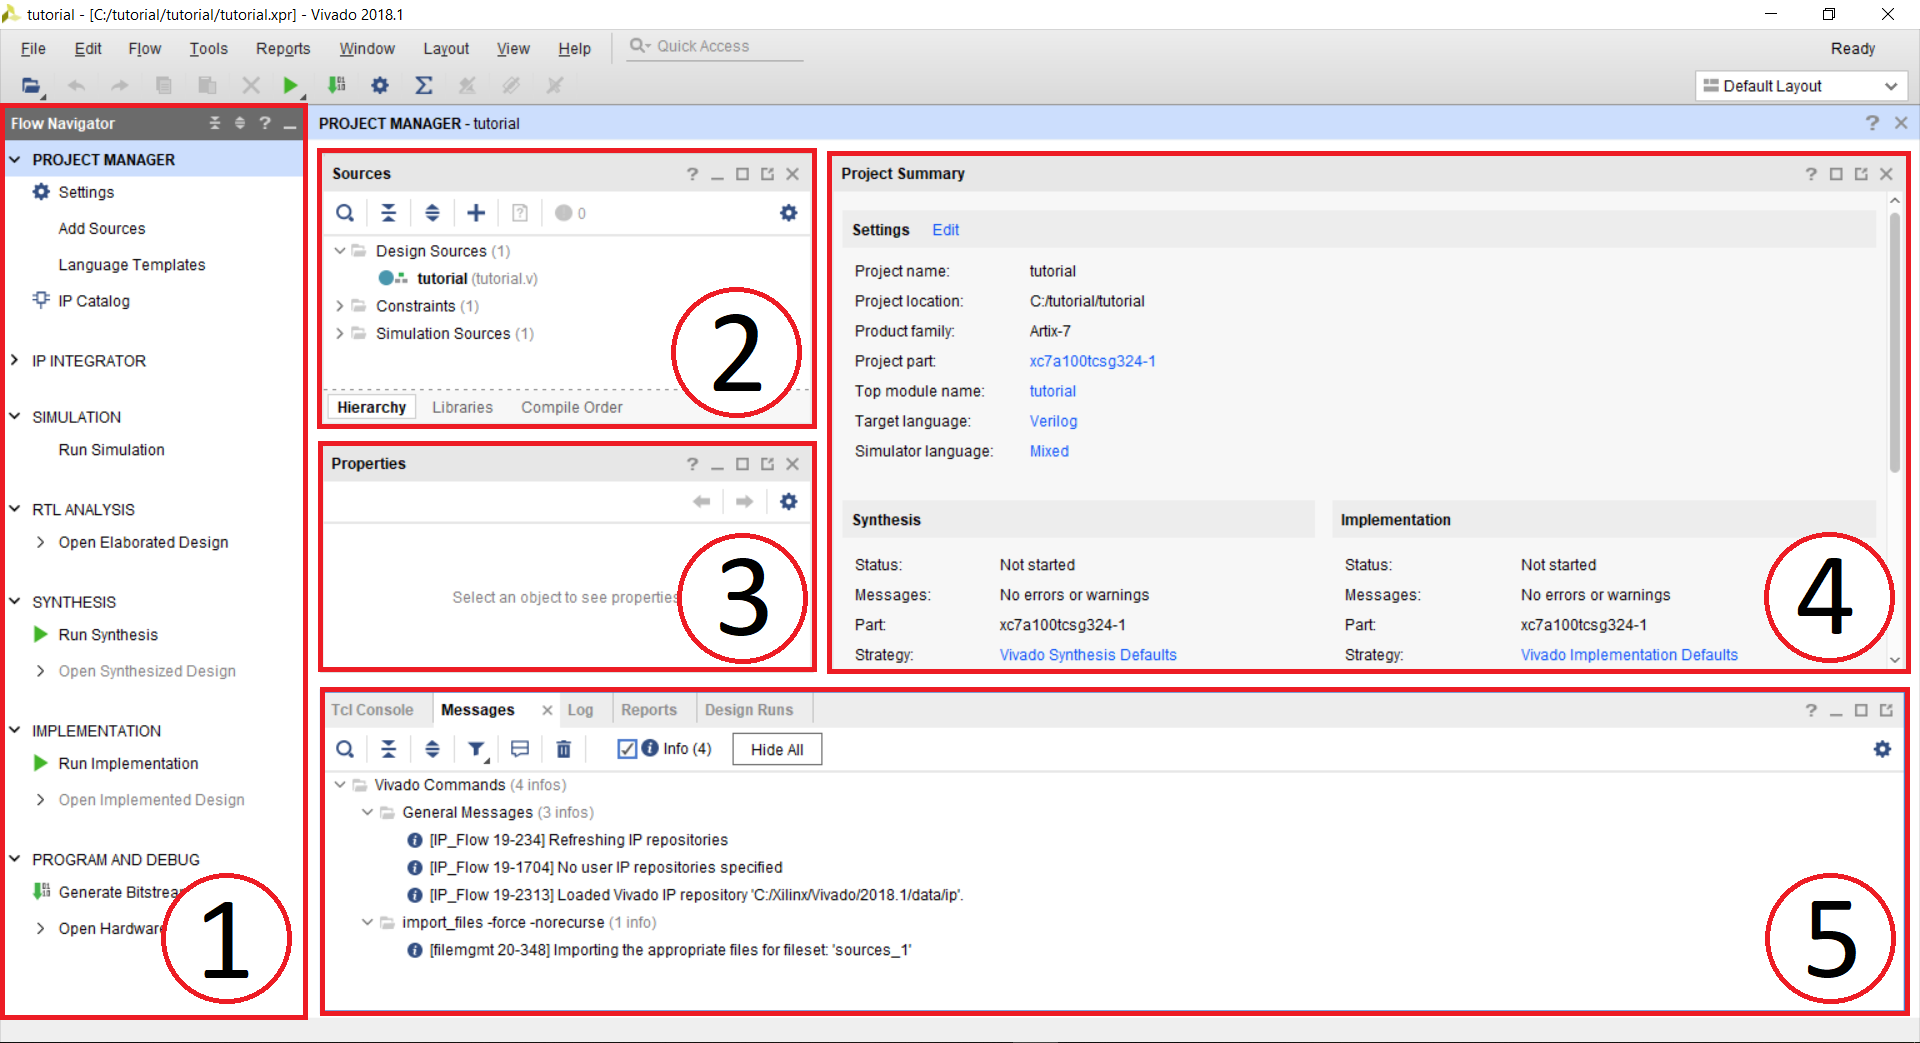
\includegraphics[width=0.9\textwidth]{images/vivado_layout.png}
    \caption{Vivado Project Manager view with panes labelled}
    \label{fig:vivado_layout}
\end{figure}

The first section, labelled with a \textbf{1}, is called the \textit{Flow Navigator}. In the \textit{Flow Navigator} you can find the various steps you would need in developing your project. For example, the \textit{Flow Navigator} has subsections for \textit{Simulation}, \textit{Synthesis}, and \textit{Implementation}. To the right of the \textit{Flow Navigator} we have various panes that make up the \textit{Project Manager} view. Note, the \textit{Flow Navigator} has actions that may open up a new view in place of the \textit{Project Manager} view. For example, the actions \textit{Open Elaborated Design}, \textit{Open Synthesized Design}, and \textit{Open Implemented Design} will open the \textit{Elaborated Design} view, the \textit{Synthesized Design} view, and the \textit{Implemented Design} view respectfully. These new views expose different information about the state of the project, and can be closed to return to the \textit{Project Manager} view (Note, closing the \textit{Project Manager} view will close the whole project).

The next section, labelled with a \textbf{2}, simply lists all of the sources included in the project. By default the \textit{Hierarchy} view is selected for the sources, which displays all of your sourced based on their connection hierarchy within the project. The \textit{top level} module in this view will be displayed in bold face. The section labelled with a \textbf{3} is the properties window and it displays the properties of whatever you have selected, such as the properties of a selected file in the Sources window.

Next, the main content window is labelled with a \textbf{4}. Here is where the contents of any open files will be displayed, and where their contents can be edited. By default, a \textit{Project Summary} page is displayed here that summarizes the current state of the project. The subsections \textit{Utilization} and \textit{Timing} are particularly useful in this summary, showing the project's utilization of the FPGA resources (which is useful to determine whether you have enough resources to implement the project) and whether the routed wires of the project have delays compatible with the clock frequencies within the project (wires with too large delays will likely cause the project to fail).

Finally, the last section, labelled with a \textbf{5}, shows various information organized in tabs. The first tab, called \textit{TCL Console}, is a console that allows Vivado commands to be issued. Vivado commands are specified in a language called TCL (hence the name TCL console), and are often used to perform advanced tasks or for scripting simpler tasks. Note, any commands you initiate with the GUI will appear in the TCL console as well. The \textit{Messages} tab shows all of the \textbf{Errors}, \textbf{Critical Warnings}, \textbf{Warnings}, and \textbf{Info Messages} for the steps run within Vivado. Generally speaking, most projects will have a very large amount of Warnings, and so we tend to focus on Errors and Critical Warnings here when we have a problem, though it is sometimes useful to comb through the Warning messages to ensure they aren't indicating an unexpected problem. The \textit{Log} tab shows the log output of the various running steps, and the \textit{Reports} tab lists all of the reports generated by the steps already run. The final tab lists the \textit{Design Runs}, though we'll likely not deviate from the default Design Runs setup in Vivado, so this tab is not that important for us.




\section{RTL Analysis}
\label{sec:rtl_analysis}
In the \textit{Sources} pane, double-click the \textbf{tutorial.v} entry to open the file in text mode. Notice in the Verilog code that the first line defines the timescale directive for the simulator. Lines 2-4 are comment lines describing the module name and the purpose of the module. Line 7 defines the beginning (marked with keyword \textbf{module}) and Line 19 defines the end of the module (marked with keyword \textbf{endmodule}). Lines 8-9 define the input and output ports whereas lines 12-17 define the actual functionality. See Figure~\ref{fig:verilog_source} for reference. Remember, any changes made to the source will only apply to the version of the source file we copied to this project (since we chose to copy source files into the project). We do not need to make any changes to the source for this tutorial.

\begin{figure}[!h]
\centering
\begin{minted}
[
frame=lines,
framesep=2mm,
baselinestretch=1.2,
bgcolor=white,
fontsize=\footnotesize,
linenos,
]
{verilog}
`timescale 1ns / 1ps
//////////////////////////////////////////////////////////////////////////////////
// Module Name: tutorial
//////////////////////////////////////////////////////////////////////////////////


module tutorial (
    input [7:0] swt,
    output [7:0] led
    );
    
    assign led[0] = ~swt[0];
    assign led[1] = swt[1] & ~swt[2];
    assign led[3] = swt[2] & swt[3];
    assign led[2] = led[1] | led[3];
    
    assign led[7:4] = swt[7:4];
    
endmodule
\end{minted}
\vspace{-0.7cm}
\caption{The Verilog source file}
\label{fig:verilog_source}
\end{figure}

In the \textit{Sources} pane, expand the \textit{Constraints} folder and double-click the \textbf{tutorial.xdc} entry to open the file in text mode. Lines 1-14 define the pin locations of the input switches [6:0] and lines 16-29 define the pin locations of the output LEDs [6:0]. The swt[7] and led[7] are deliberately not defined so you can learn how to enter them using other methods later in the tutorial.

Now that we have our sources setup and are happy with their contents, we can see what hardware will be generated from the source. Expand the \textit{Open Elaborated Design} entry under the \textit{RTL Analysis} tasks of the \textit{Flow Navigator}
pane and click on \textbf{Schematic}. Click \textbf{OK} on any pop-ups that come up. The model (design) will be elaborated and the \textit{Elaborated Design} view will be opened with a logic view of the design displayed. See Figure~\ref{fig:schem} for the logic view that we expect. Notice that some of the switch inputs go through gates before being output to LEDs and the rest go straight through to LEDs (through I/O buffers) as modeled in the file.

\begin{figure}[!h]
    \centering
    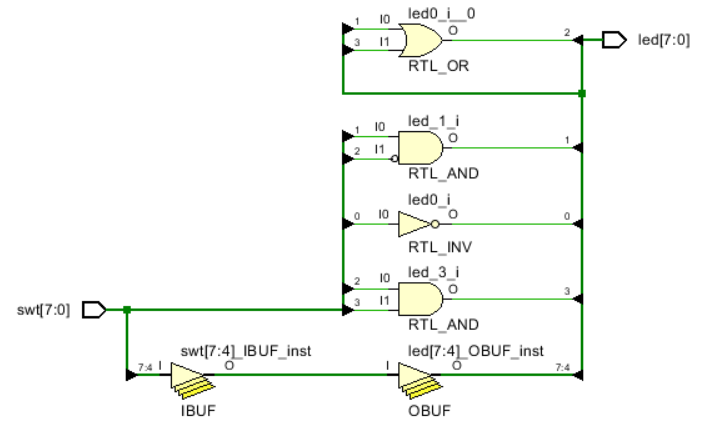
\includegraphics[width=0.9\textwidth]{images/schematic.png}
    \caption{The schematic created from the elaborated design}
    \label{fig:schem}
\end{figure}




\section{Adding I/O Constraints}
\label{sec:add_cons}
In Section~\ref{sec:rtl_analysis} we noted that we had some missing constraints in our project. The pin locations for led[6:0] and swt[6:0] are defined in our \textit{constraints.xdc}; we could add the constraints for pins led[7] and swt[7] to that file, though for the sake of demonstration we'll go over a number of other ways to add pin constraints to a project.

Once RTL analysis is performed and we have our \textit{Elaborated Design} view open, another standard layout called the I/O Planning layout is available. Click on the drop-down list on the top-right of the Vivado interface and select the I/O Planning layout. See Figure~\ref{fig:io_plan} for details. Notice that the \textit{Package} view is displayed in the Content View area and the \textit{I/O ports} tab is displayed in the Console View area at the bottom of the Vivado interface. Also notice that design ports (led and swt) are listed in the I/O Ports tab with both having multiple I/O standards.

\begin{figure}[!h]
    \centering
    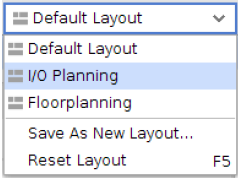
\includegraphics[width=0.3\textwidth]{images/io_plan.png}
    \caption{The Layout dropdown menu}
    \label{fig:io_plan}
\end{figure}

Move the mouse cursor over the Package view, highlighting different pins. Notice the pin site number is shown at the bottom of the Vivado GUI, along with the pin type (User IO, GND, VCCO…) and the I/O bank it belongs to (See Figure~\ref{fig:io_sites}). 

\begin{figure}[!h]
    \centering
    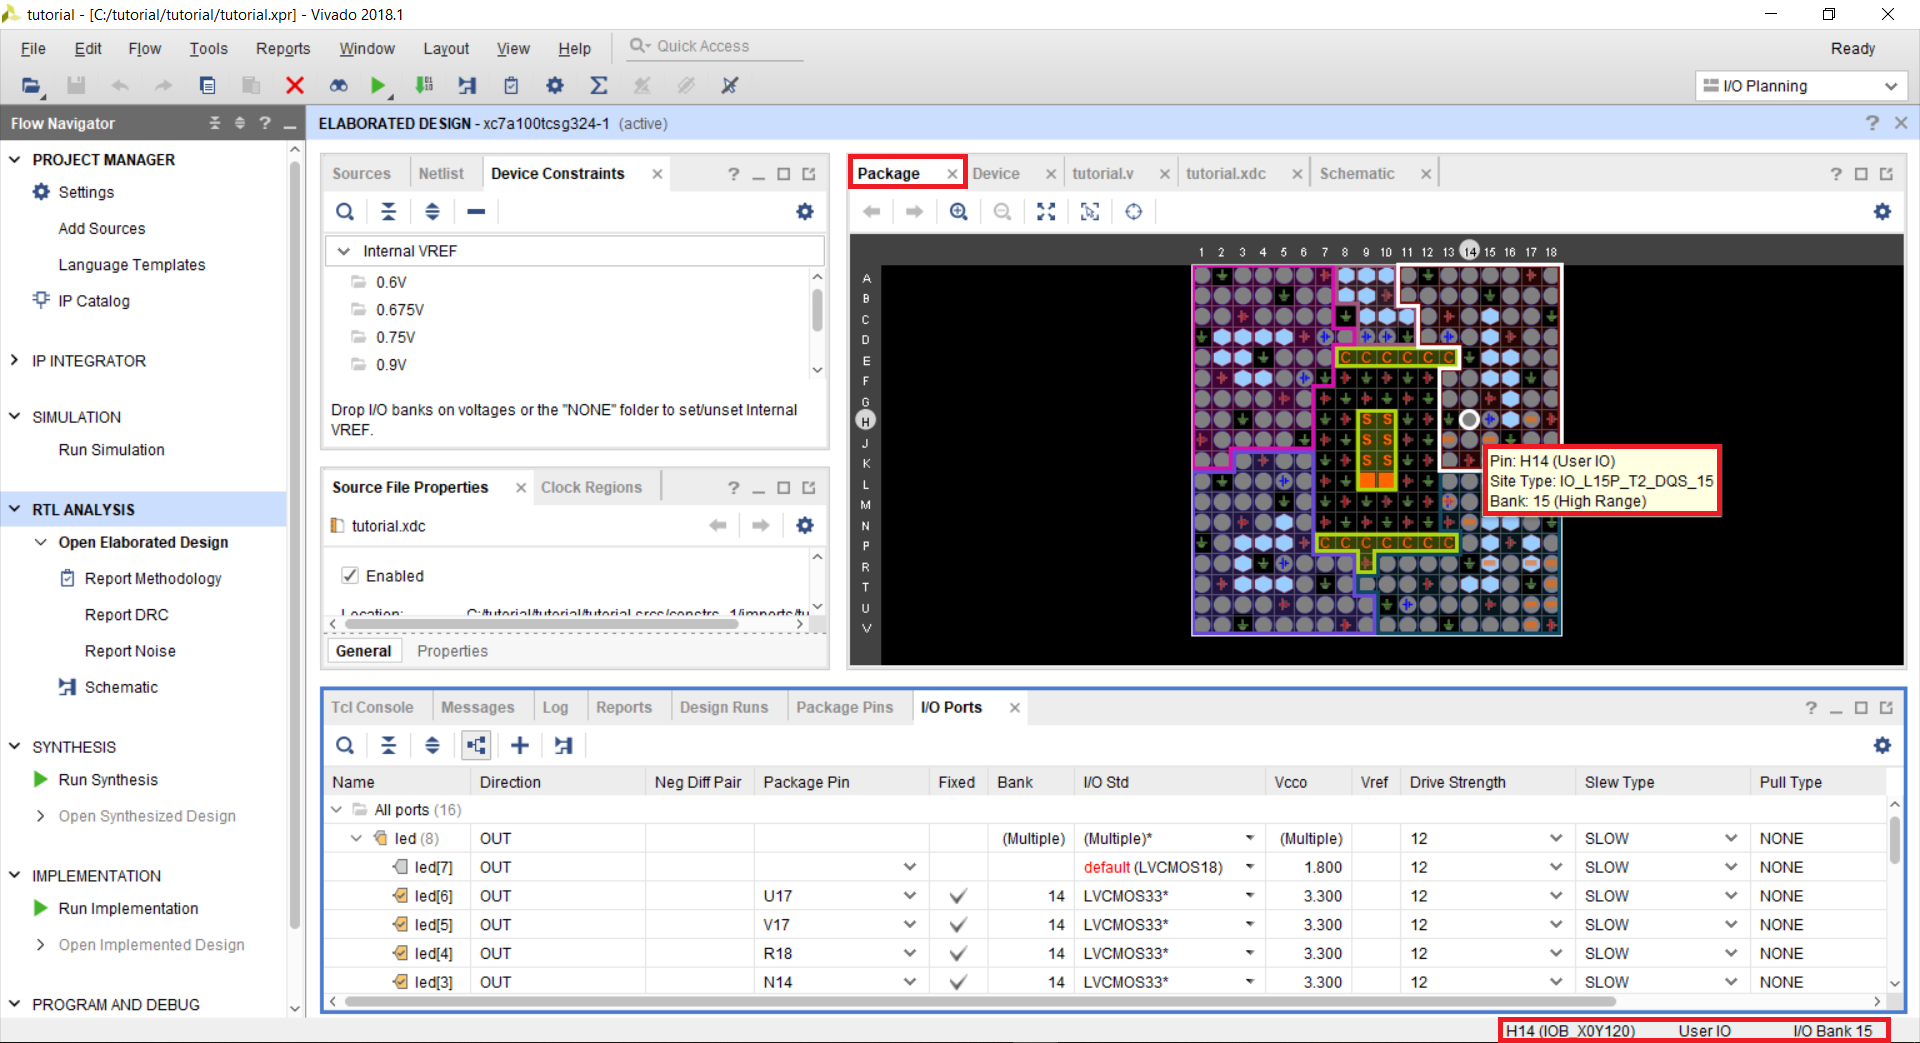
\includegraphics[width=\textwidth]{images/io_sites.png}
    \caption{The Package view with some IO site highlighted}
    \label{fig:io_sites}
\end{figure}

Expand the \textbf{led} and \textbf{swt} ports by clicking on the + box and observe that led [6:0] and swt[6:0] have assigned pins and uses the LVCMOS33 I/O standard whereas led[7] and swt[7] do not have assigned pins and defaults to LVCMOS18; hence you can see multiple I/O standard in the collapsed view (see Figure~\ref{fig:io_expand}). 

\begin{figure}[!h]
    \centering
    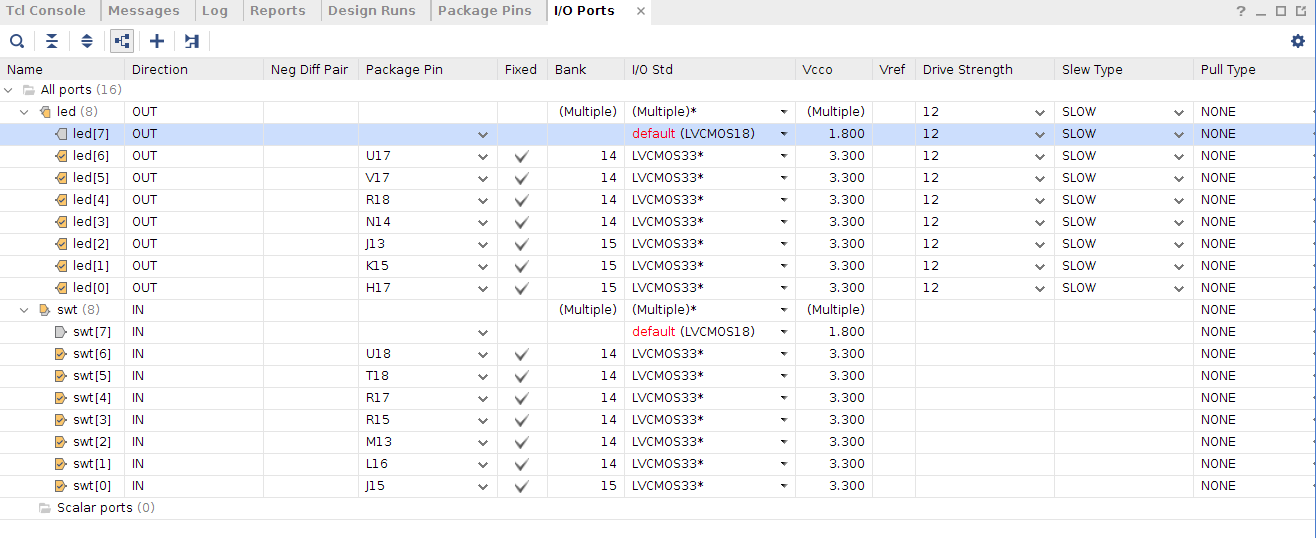
\includegraphics[width=\textwidth]{images/io_expand.png}
    \caption{The pin sites assigned to each of the top level signals}
    \label{fig:io_expand}
\end{figure}

Click under the \textit{Package Pin} column across \textbf{led[7]} row to see a drop-down box appear. Type U in the field to jump to Uxx pins, scroll-down until you see U16, select U16 and hit the \textbf{Enter} key to assign the pin. Notice after selecting the pin U16, the Package Pin column automatically places \textbf{led[7]} lower down in the column since it alphabetically arranges the site/pin names. Similarly, click under the \textit{I/O Std} column across the \textbf{led[7]} row and select LVCMOS33. This assigns the LVCMOS33 standard to the site. We have now assigned a pin location using the \textit{I/O Planning} methodology, though you can also assign pins using TCL commands. Open the TCL Console and type the following commands to select the pin and I/O standard for \textbf{swt[7]}:

\begin{verbatim}
    set_property package_pin R13 [get_ports {swt[7]}]
    set_property iostandard LVCMOS33 [get_ports [list {swt[7]}]]
\end{verbatim}

\noindent
Observe the pin and I/O standard assignments changed in the I/O Ports tab. 

Finally, You can also assign the pin constraints by selecting its entry (swt[7]) in the I/O ports tab, and dragging it to the Package view, and placing it at the \textbf{R13} location. You can assign the LVCMOS33 standard by selecting its entry (swt[7]), selecting the \textit{Configure} tab of the I/O Port Properties window, followed by clicking the drop-down button of the I/O standard field, and selecting LVCMOS33 (see Figure~\ref{fig:io_std}).

\begin{figure}[!h]
    \centering
    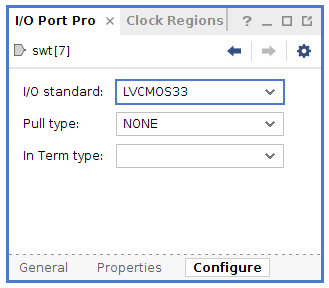
\includegraphics[width=0.5\textwidth]{images/io_std.png}
    \caption{Selecting the IO Standard in the pin property window}
    \label{fig:io_std}
\end{figure}

Once we have assigned all of our pin locations, we can save our assignments to the \textit{tutorial.xdc} file. Select save on upper left part of Vivado to save the constraints in the \textit{tutorial.xdc} file. Click \textbf{Update} when warning is prompted. Note, the changes were made to the project's local copy of the \textit{constraints.xdc} file. Close the \textit{Elaborated Design} view to return to the \textit{Project Manager}.




\section{Simulating with XSim}
\label{sec:simulation}
We usually want to test our projects using the Vivado simulator before synthesizing the project and downloading the project to the board. In order to test the project we use a testbench, which is simply a Verilog source file designed to test our project. Click \textbf{Add Sources} under the \textit{Project Manager} tasks of the \textit{Flow Navigator} pane. Select the \textit{Add or Create Simulation Sources} option and click \textbf{Next} (See Figure~\ref{fig:add_tb}). In the \textit{Add Source Files} form, click the \textbf{Add Files…} button. Navigate to the directory to which you extracted the files and select \textit{tutorial\_tb.v} and click \textbf{OK} and then click \textbf{Finish}. In the \textit{Sources} pane, the hierarchy under \textit{Design Sources} should remain unchanged, though if you expand the \textit{Simulation Sources} folder, you should now see a \textit{tutorial\_tb} module under which the \textit{tutorial} module is instantiated, as per Figure~\ref{fig:tb_hier}.

\begin{figure}[!h]
    \centering
    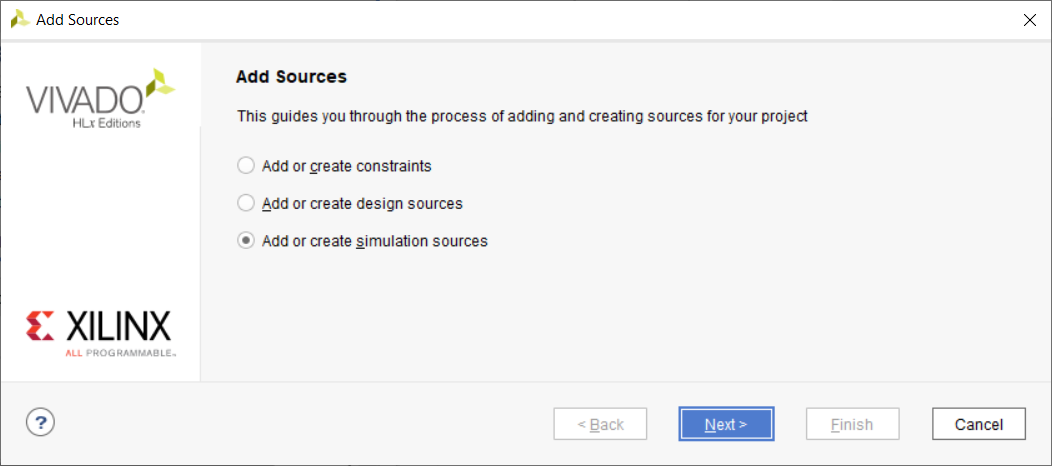
\includegraphics[width=0.9\textwidth]{images/add_tb.png}
    \caption{Adding simulation sources to the project}
    \label{fig:add_tb}
\end{figure}

\begin{figure}[!h]
    \centering
    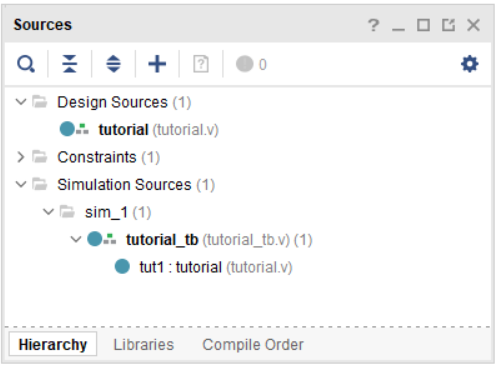
\includegraphics[width=0.5\textwidth]{images/tb_hier.png}
    \caption{Source hierarchy after adding a testbench}
    \label{fig:tb_hier}
\end{figure}

Double-click on the \textbf{tutorial\_tb} in the Sources pane to view its contents. The testbench defines the simulation step size and the resolution in line 1. The testbench module definition begins on line 5. Line 15 instantiates the DUT (device/module under test). Lines 17 through 26 define the same module functionality for the expected value computation. Lines 28 through 39 define the stimuli generation and compares the expected output with what the DUT provides. Line 41 ends the testbench. The \$display task will print the message in the simulator console window when the simulation is run.

Before running the simulation, let's set some of the simulation settings. Right Click \textbf{Simulation} in the Flow Navigator pane and select Simulation Settings. A \textit{Settings} form will appear showing the \textit{Simulation} properties form. Select the Simulation tab, and set the \textbf{Simulation Run Time} value to 200 ns and click \textbf{OK} (See Figure~\ref{fig:sim_settings}). Click on \textbf{Run Simulation $\rightarrow$ Run Behavioral Simulation} under the \textit{Simulation} tasks of the \textit{Flow Navigator} pane. The testbench and source files will be compiled and the XSim simulator will be run (assuming no errors). 

\begin{figure}[!h]
    \centering
    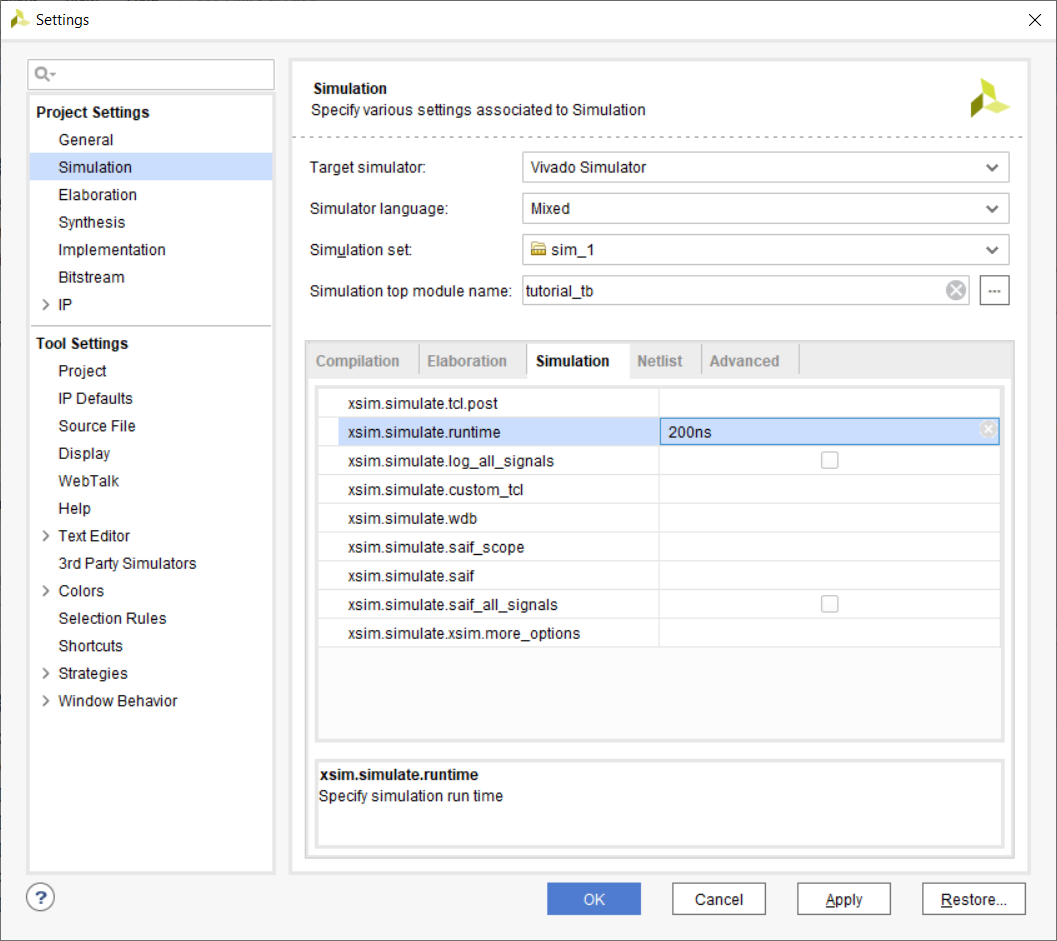
\includegraphics[width=0.9\textwidth]{images/sim_settings.png}
    \caption{Changing the simulation settings}
    \label{fig:sim_settings}
\end{figure}

You will see a simulator output similar to the one shown in Figure~\ref{fig:sim_output}. You will see four main views: (i) Scopes, where the testbench hierarchy as well as global instances are displayed, (ii) Objects, where top-level signals are displayed, (iii) the waveform window, and (iv) the TCL Console where the simulation outputs are displayed. Notice that since the testbench used is self-checking, the results are displayed as the simulation is run. 

Click on the \textbf{Zoom Fit} button
(\scalerel*{
\includegraphics{images/zoom_fit.png}}{(})
located above the waveform window to see the entire waveform within the current waveform window. Also, to get a better view of the waveform, you can click the \textbf{Float button} in the top-right-most corner of the waveform window to detach the waveform window from the rest of the simulation view and re-size it independently. Figure~\ref{fig:sim_wave} shows the expected waveform output from our simulation.

\begin{figure}[!h]
    \centering
    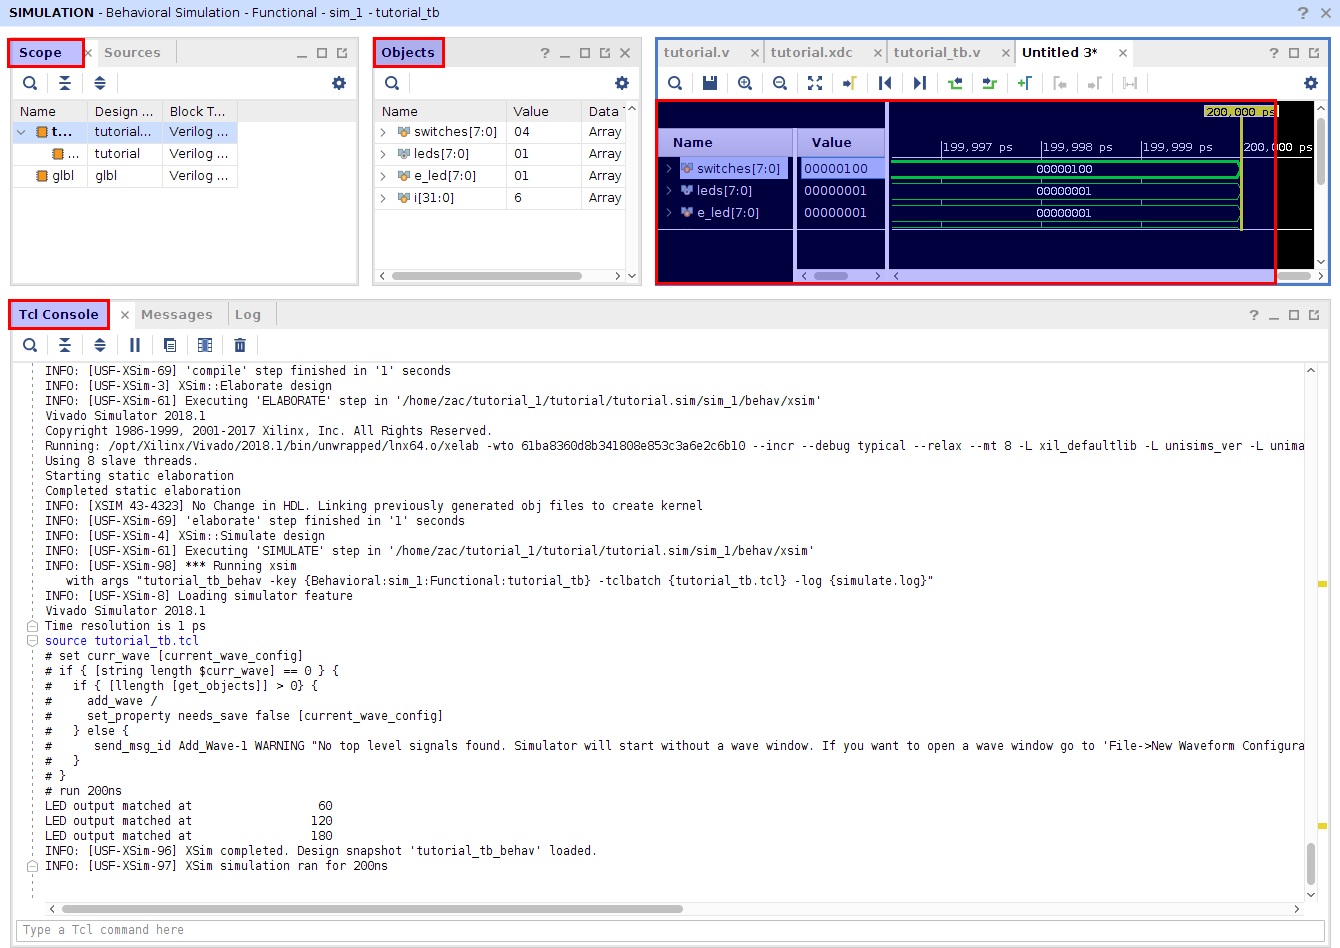
\includegraphics[width=\textwidth]{images/sim_output.png}
    \caption{Simulator output}
    \label{fig:sim_output}
\end{figure}

\begin{figure}[!h]
    \centering
    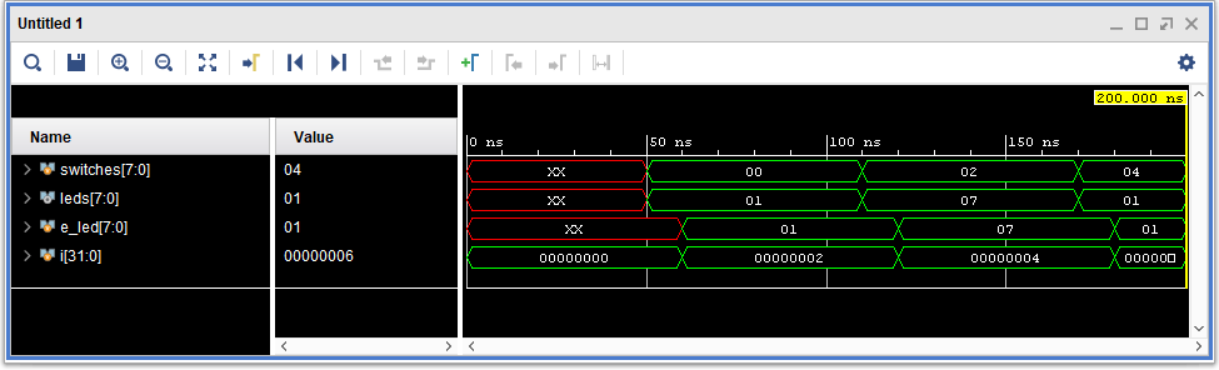
\includegraphics[width=\textwidth]{images/sim_wave.png}
    \caption{Simulator waveform}
    \label{fig:sim_wave}
\end{figure}


Within the wavefrom viewer, there are a number of things we can change to make it easier to examine the output. Select \textbf{i[31:0]} in the waveform window, right-click, select \textbf{Radix}, and then select \textit{Unsigned Decimal} to view the for-loop index in integer form. Similarly, change the radix of \textbf{switches[7:0]} to \textit{Hexadecimal}. Finally, change the radix for the \textbf{leds[7:0]} and \textbf{e\_led[7:0]} to binary as we want to see each output bit. 
\\
\\

We can also add more signals to the waveform viewer for monitoring. Expand the tutorial\_tb instance, if necessary, in the \textit{Scopes} window and select the tut1 instance. The swt[7:0] and led[7:0] signals will be displayed in the \textit{Objects} window (see Figure~\ref{fig:sim_scope}). Select \textbf{swt[7:0]} and \textbf{led[7:0]} and drag them into the waveform window to monitor those lower-level signals.
\\
\\

\begin{figure}[!h]
    \centering
    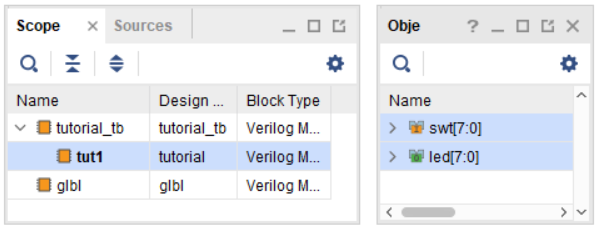
\includegraphics[width=0.7\textwidth]{images/sim_scope.png}
    \caption{Simulator Scopes and Objects windows}
    \label{fig:sim_scope}
\end{figure}

In order to see values for our newly added signals, we need to run the simulator again. To do this, examine the simulator ribbon bar. Specifically, the buttons in Figure~\ref{fig:sim_button} are of note. The first button rewinds the simulation to time zero; if we want to rerun the simulation, we must rewind it first. Next, the play button will run the simulator indefinitely until it receives a stop signal or the testbench has nothing else to do; for most uses cases this is not useful (unless we explicitly have a \$finish command in our testbench) as it will cause the simulator to run forever. Finally, the play button annotated with a (T) will run the simulator for an additional amount of time, specified in the entry box beside it. \textbf{Enter} the value 500ns into the box, press the \textbf{Rewind} button, and then press the \textbf{Timed Start} button to rerun the simulator for 500ns from time zero. We expect to see the waveform from Figure~\ref{fig:sim_wave2} (remember to press the \textbf{Zoom Fit} button to fit the entire waveform in the window).

\begin{figure}[!h]
    \centering
    
\includegraphics[width=0.4\textwidth]{images/sim_button.png}
    \caption{Simulator ribbon bar to control simulation}
    \label{fig:sim_button}
\end{figure}

\begin{figure}[!h]
    \centering
    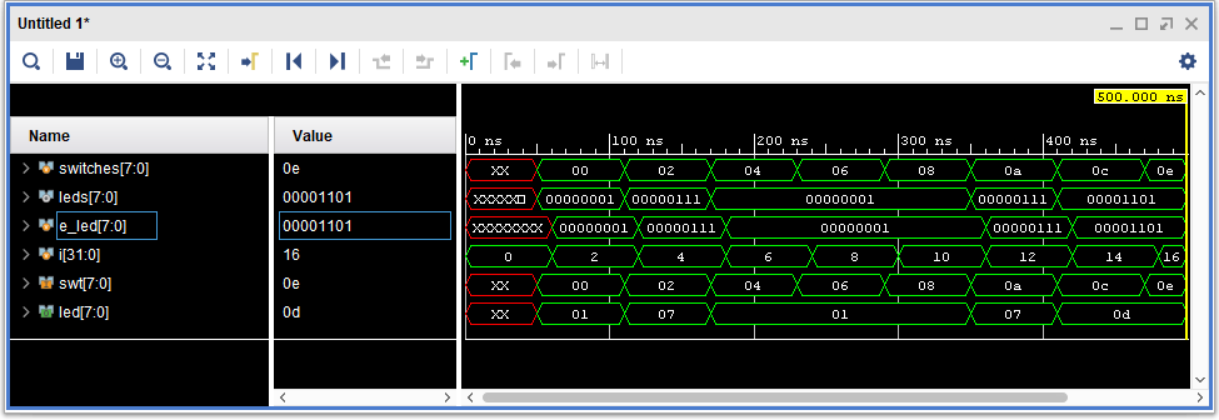
\includegraphics[width=\textwidth]{images/sim_wave2.png}
    \caption{Simulator waveform updated}
    \label{fig:sim_wave2}
\end{figure}

\noindent
Close the simulator by selecting \textbf{File $\rightarrow$ Close Simulation}. Click \textbf{OK} and then click \textbf{Discard} to close without saving the waveform.




\section{Design Synthesis}
\label{sec:synthesis}
Click on \textbf{Run Synthesis} under the \textit{Synthesis} tasks of the \textit{Flow Navigator} pane and then click \textbf{OK} to start the synthesis process. The synthesis process will be run on the \textit{tutorial.v} file (and all its hierarchical files if they exist). When the process is completed a \textit{Synthesis Completed} dialog box with three options will be displayed. Usually we would proceed to the \textbf{Run Implementation}, though we don't want to run the implementation yet, so press \textbf{Cancel} rather then selecting any of the three options.

Open the \textit{Project Summary} page to see summarized information from the synthesis run. The main information we're generally interested in after synthesis is the utilization, so scroll down to that section of the summary. Click on the \textbf{Table} tab to see the utilization results in tabular form. We notice that our project requires 3 LUTs and 16 IOs (see Figure~\ref{fig:util}), which represents a very low amount of of the total resources available on our FPGA (only 0.01\% of the LUTs).

\begin{figure}[!h]
    \centering
    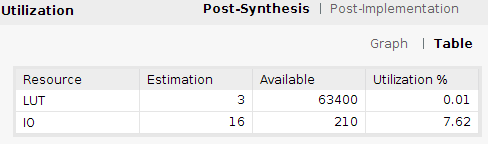
\includegraphics[width=0.6\textwidth]{images/util.png}
    \caption{Post-synthesis utilization results}
    \label{fig:util}
\end{figure}

Next, we can take a look at the post-synthesis schematic of our design. Click on \textbf{Schematic} under the \textit{Open Synthesized Design} of \textit{Synthesis} tasks of the Flow Navigator pane to view the synthesized design in a schematic view. This will open the \textit{Synthesized Design} view and then bring up the schematic of the synthesized design (see Figure~\ref{fig:schem2}). Notice that IBUF and OBUF are automatically instantiated (added) to the design as the inputs and outputs are buffered. The logical gates are implemented in LUTs (1 input LUTs are listed as LUT1, 2 input LUTs are listed as LUT2, and 3 input LUTs are listed as LUT3). The four gates from the RTL analysis schematic (Figure~\ref{fig:schem}) are mapped to four LUTs in this synthesized output. Close the \textit{Synthesized Design} view to return to thr \textit{Project Manager}.
\newpage

\begin{figure}[!h]
    \centering
    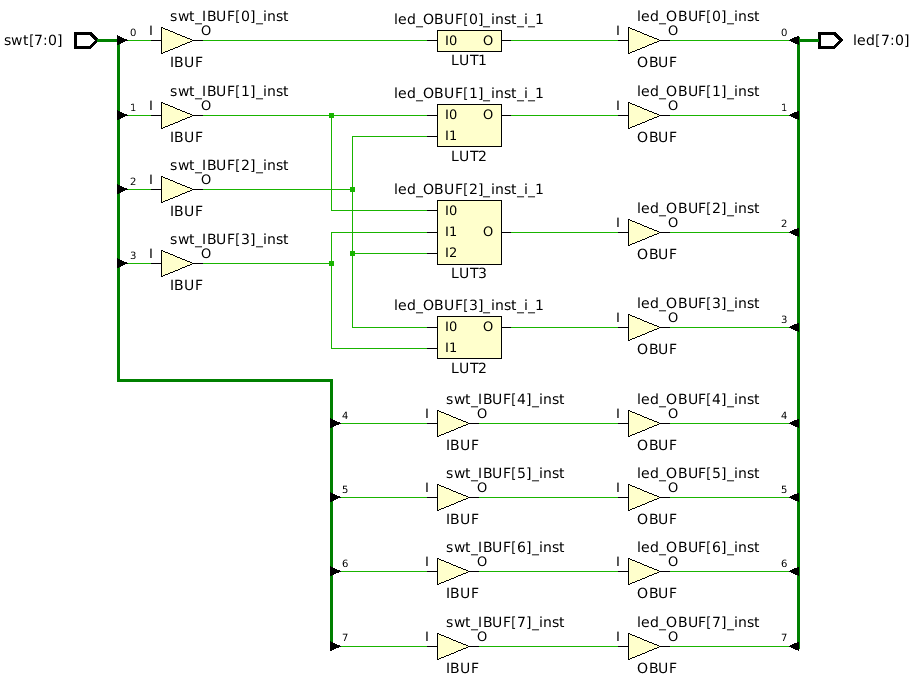
\includegraphics[width=0.9\textwidth]{images/schem_post_syn.png}
    \caption{Post-synthesis schematic}
    \label{fig:schem2}
\end{figure}




\section{Design Implementation}
\label{sec:impl}
Click on \textbf{Run Implementation} under the \textit{Implementation} tasks of the \textit{Flow Navigator} pane and then click \textbf{OK} to start the implementation process. The implementation process will run on the results of the synthesis. When the process is completed a \textit{Implementation Completed} dialog box with three options will be displayed. Select \textit{Open implemented design} and click \textbf{OK} as we want to look at the implemented design in a Device view tab. The \textit{Implemented Design} view will be opened.

In the \textit{Netlist} pane on the left side, select one of the nets (e.g. led\_OBUF[1]) and notice the net displayed in the Device view tab (you may have to zoom in to see it). Here we can see the wire used to route that net in the device. This can be done for any net in your design. In addition, under the \textit{Leaf Cells} section in the \textit{Netlist} pane, you can select any of the nodes in your design to see where it was placed. See Figure~\ref{fig:net_route} for an example of a routed net displayed on the \textit{Device} view.

\begin{figure}[!h]
    \centering
    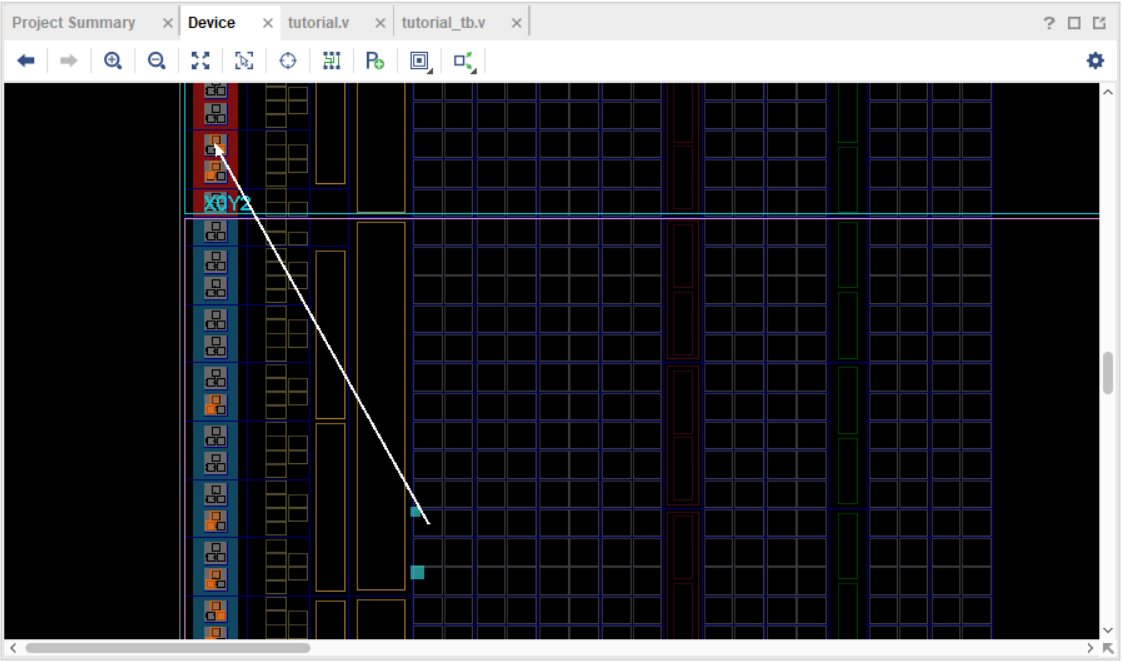
\includegraphics[width=0.9\textwidth]{images/net_route.png}
    \caption{Routed net shown in Implemented Design Device view}
    \label{fig:net_route}
\end{figure}

Close the \textit{Implemented Design} view  to return to the \textit{Project Manager}. Select the \textit{Project Summary} tab to see the summarized information from the implementation run. In general, we're interested is viewing the post-implementation utilization results (i.e. the final actual utilization) and the timing report summary. First, the timing report should have no information since we don't have any clocks or sequential elements in our design. Looking at the utilization results, we can again look at the utilization \textit{Table} view to see that 3 LUTs and 16 IOs are used. The utilization hasn't changed since synthesis, since the design is pretty simple, though often there is some change in utilization once implementation is run due to additional optimization passes and other factors in implementation. Note, under \textit{Implementation} in the \textit{Flow Navigator}, when you expand \textit{Open Implemented Design}, there are options to get more detailed reports for both timing and utilization, which may be helpful in future projects.




\section{Timing Simulation with XSim}
\label{sec:timing_sim}
Select the \textbf{Run Simulation $\rightarrow$ Run Post-Implementation Timing Simulation} process under the \textit{Simulation} section of the \textit{Flow Navigator} pane. The XSim simulator will be launched using the implemented design and tutorial\_tb as the top-level module. This simulation is different than the one presented in Section~\ref{sec:simulation} as it considers the real delays of the routed design produced by the implementation run. Click on the \textbf{Zoom Fit} button to see the waveform window from 0 to 200 ns.

We can add markers to the waveform to allow us to more easily see the relative difference between signals. \textbf{Right-click} at 50ns (where the switch input is set to 0000000b) and select \textbf{Markers $\rightarrow$ Add Marker}. Similarly, right-click and add a marker at around 55ns where the \textbf{leds} complete their transition. You can also add a marker by clicking on the Add Marker button 
(\scalerel*{
\includegraphics{images/add_mark.png}}{(})
. Click on the \textbf{Add Marker} button and left-click at around 60ns where e\_led changes. Note that the leds change 5ns after the input swt changes, which represents the actual delays of our IBUF, OBUF, and net routing. Close the simulation by selecting \textbf{File $\rightarrow$ Close Simulation}; there is no need to save the waveform.




\section{Bitsream Generation and Verification on Device}
\label{sec:bitgen}
Click on the \textbf{Generate Bitstream} entry under the \textit{Program and Debug} tasks of the \textit{Flow Navigator} pane. The bitstream generation process will be run on the implemented design. The process will create a \textit{tutorial.bit} file in the \textit{impl\_1} directory of the \textit{tutorial.runs} directory within your project folder. When the process is completed a \textit{Bitstream Generation Completed} dialog box with four options will be displayed. If you are ready to program the device, select \textit{Open Hardware Manager} and click \textbf{OK}, otherwise click \textbf{Cancel}. As long as you have your board ready, you should opt to \textit{Open Hardware Manager}.

The board can be powered by USB or the external power jack. Since we are connecting the USB in order to program the board, we can use this as the power source, though we need to change the \textit{Power Select} jumper on the board to the \textit{USB} setting in order to allow this. If you'd rather leave the board powered through the power jack, leave the jumper and make sure to plug in the board's power. Connect the provided micro-USB cable between the board's \textit{JTAG Programming} port and the PC and power \textbf{ON} the board. See Figure~\ref{fig:board_power} for reference.

\begin{figure}[!h]
    \centering
    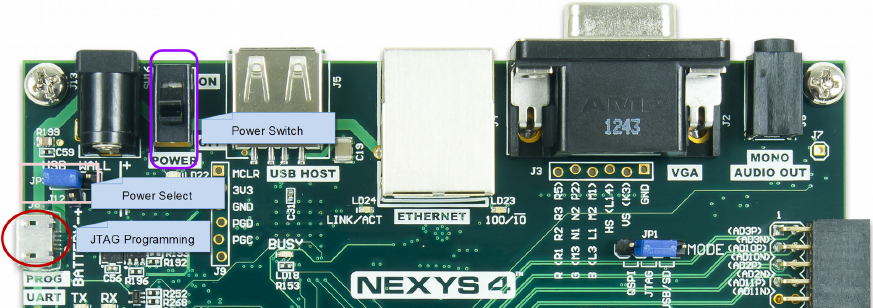
\includegraphics[width=0.9\textwidth]{images/board_power.png}
    \caption{Board power configuration and programming/power port locations}
    \label{fig:board_power}
\end{figure}

The Hardware Manager window will open indicating “unconnected” status. Click on the \textbf{Open target} link and \textbf{Auto Connect} (see Figure~\ref{fig:auto_connect}). Select the \textit{Program device} link and click on the FPGA part \textbf{xc7a100t\_0}. A dialog will appear showing the path to the bitstream file; by default the prompt will point to the bistream file we just generated. Click \textbf{Program} to program the FPGA. The DONE light on the FPGA will be lit when the device is programmed.

\begin{figure}[!h]
    \centering
    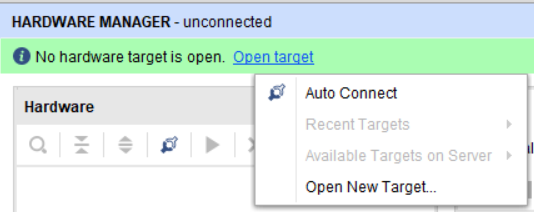
\includegraphics[width=0.7\textwidth]{images/auto_connect.png}
    \caption{Auto connect to board from Hardware Manager}
    \label{fig:auto_connect}
\end{figure}

Verify the functionality by flipping switches and observing the output on the LEDs. When satisfied, power \textbf{OFF} the board. Close the hardware session by selecting \textbf{File $\rightarrow$ Close Hardware Manager}. Click \textbf{OK} to close the session. Close the Vivado program by selecting \textbf{File $\rightarrow$ Exit} and click \textbf{OK}.




\section{Running Vivado in Batch Mode} 
\label{sec:batch_mode}
In the previous sections we have run Vivado in what is called \textit{Project Mode}. You can also run Vivado in \textit{Batch Mode}, where Vivado is given a TCL script and simply runs the steps specified in that TCL script. Batch mode is run from the terminal (or Command Prompt on Windows), so first \textbf{open} a Terminal (or Command Prompt) session. From Section~\ref{sec:create_proj} recall that we need to source a specific script file in order to use Vivado, follow those steps to do so. Next, change to the directory where you extracted the tutorial files. In this directory you should see a TCL file called \textit{tutorial\_tcl\_with\_sim.tcl}. 

The contents of this TCL file are shown in Figure~\ref{fig:tcl}. Line 1 sets the output directory path; line 2 creates the project directory tutorial\_tcl\_with\_sim under the \$outDir directory targeting the Artix-7 100 part; line 3 adds the source file; line 4 imports the constraints files; line 5 sets the top module file; line 6 executes the rtl analysis command; lines 7 through 10 add the missing I/O pins constraints; lines 11 through 13 save the constraints in the target xdc file; lines 14 through 17 set up, read, and compile the testbench; line 18 runs the behavioral simulation; lines 19 through 22 synthesizes and implements the design; and line 23 generates the bitstream. Note that wait\_on\_run on lines 20 and 22 are essential as the results from the steps that precede them are needed before executing the next command.

\begin{figure}[!h]
\centering
\begin{minted}
[
frame=lines,
framesep=2mm,
baselinestretch=1.2,
bgcolor=white,
fontsize=\footnotesize,
linenos,
breaklines,
]
{tcl}
set outDir .
create_project tutorial_tcl_with_sim $outDir/tutorial_tcl_with_sim -part xc7a100tcsg324-1
add_files -norecurse $outDir/tutorial.v
import_files -fileset constrs_1 -force -norecurse $outDir/tutorial.xdc
update_compile_order -fileset sources_1
synth_design -rtl -name rtl_1
set_property package_pin U16 [get_ports {led[7]}]
set_property iostandard LVCMOS33 [get_ports [list {led[7]}]]
set_property package_pin R13 [get_ports {swt[7]}]
set_property iostandard LVCMOS33 [get_ports [list {swt[7]}]]
set_property target_constrs_file \
$outDir/tutorial_tcl_with_sim/tutorial_tcl_with_sim.srcs/constrs_1/imports/tutorial_1/tutorial.xdc [current_fileset -constrset]
save_constraints -force
set_property SOURCE_SET sources_1 [get_filesets sim_1]
import_files -fileset sim_1 -norecurse $outDir/tutorial_tb.v
update_compile_order -fileset sim_1
set_property runtime 200ns [get_filesets sim_1]
launch_simulation -simset sim_1 -mode behavioral
launch_runs synth_1
wait_on_run synth_1
launch_runs impl_1
wait_on_run impl_1
launch_runs impl_1 -to_step write_bitstream
wait_on_run impl_1
\end{minted}
\vspace{-0.7cm}
\caption{The TCL script for batch mode}
\label{fig:tcl}
\end{figure}

To run Vivado in batch mode using this script, type the following command into the terminal or command prompt:

\begin{verbatim}
    vivado –mode batch –source tutorial_tcl_with_sim.tcl
\end{verbatim}

\noindent
The tools will be run and various directories will be created. Note that there may be some errors due to files that cannot be found. This could occur depending on the original directory names where the script is invoked and where sources are found. If the errors occur, it should be clear what paths are incorrect and the script can be modified accordingly. Once the script is done executing, you can close the terminal and examine the generated folder structures.




\section{Summary}
\label{sec:summary}
The Vivado software tools can be used to perform a complete design flow. The project was created using the supplied source files (HDL model and user constraint file). A behavioral simulation was done to verify the model functionality. The model was then synthesized, implemented, and a bitstream was generated. The timing simulation was run on the implemented design using the same testbench. The functionality was verified in hardware using the generated bitstream. The design flow was also carried out in batch mode using the provided TCL script.




%\newpage
%S\printbibliography

\end{document}
